\documentclass{report}
\usepackage{tikz}
\usetikzlibrary{calc}

\begin{document}

\begin{tikzpicture}[line join=round,scale=1.1]
	\foreach \x in {0,3,6,9,12,15}
	\draw[line width=1pt,pink] (0,\x) -- (9,\x);
	\foreach \x in {0,3,6,9}
	\draw[line width=1pt,pink] (\x,0) -- (\x,15);
	\draw[line width=1pt,pink] (0,0) -- (9,0) -- (9,15) -- (0,15) -- cycle;

	\foreach \x in {0,3,6}
	\foreach \y in {3,6,...,15}
	\draw[pink,line width=1pt] (\x,\y-.3) rectangle (\x+.3,\y);


	\draw[pink,line width=1pt] (.15,2.85)  node {\tiny $1$};
	\draw[pink,line width=1pt] (3.15,2.85)  node {\tiny $2$};
	\draw[pink,line width=1pt] (6.15,2.85)  node {\tiny $3$};


	\draw[pink,line width=1pt] (.15,5.85)  node {\tiny $4$};
	\draw[pink,line width=1pt] (3.15,5.85)  node {\tiny $5$};
	\draw[pink,line width=1pt] (6.15,5.85)  node {\tiny $6$};

	\draw[pink,line width=1pt] (.15,8.85)  node {\tiny $7$};
	\draw[pink,line width=1pt] (3.15,8.85)  node {\tiny $8$};
	\draw[pink,line width=1pt] (6.15,8.85)  node {\tiny $9$};

	\draw[pink,line width=1pt] (.15,11.85)  node {\tiny $10$};
	\draw[pink,line width=1pt] (3.15,11.85)  node {\tiny $11$};
	\draw[pink,line width=1pt] (6.15,11.85)  node {\tiny $12$};

	\draw[pink,line width=1pt] (.15,14.85)  node {\tiny $13$};
	\draw[pink,line width=1pt] (3.15,14.85)  node {\tiny $14$};
	\draw[pink,line width=1pt] (6.15,14.85)  node {\tiny $15$};


	\draw (1.5,1.5) node {
		%%%%%%Pentagon Type 1
		\begin{tikzpicture}[line join=round,line width=1.2pt,scale=.5]
			\begin{tiny}
				\draw (0,0) coordinate (A) node[below] {$A$};
				\draw ($ (A) + (15:27mm) $) coordinate (B) node[right] {$B$};
				\draw ($(B)!26mm!-67:(A)$) coordinate (C) node[above] {$C$};
				\draw ($(C)!11mm!-113:(B)$) coordinate (D) node [left] {$D$};
				\draw ($(D)!17mm!-125:(C)$) coordinate (E) node [left] {$E$};

				\draw[fill=yellow!20,yellow!20] (A) -- (B) -- (C) -- (D) -- (E) -- cycle;


				\draw [pink] (A) -- (B) node[pos=.5,below] {$b$};
				\draw [blue](B) -- (C) node[pos=.5,above right] {$c$};
				\draw [green](C) -- (D) node[pos=.5,above] {$d$};
				\draw (D) -- (E) node[pos=.5,left] {$e$};
				\draw[red](E) -- (A) node[pos=.5,below left] {$a$};

				\draw[fill] (A) circle (.6pt);
				\draw[fill] (B) circle (.6pt);
				\draw[fill] (C) circle (.6pt);
				\draw[fill] (D) circle (.6pt);
				\draw[fill] (E) circle (.6pt);


				\draw (1,-.9) node{$\widehat{B}+\widehat{C}=180^\circ$};
				\draw (1,-1.5) node{$\widehat{A}+\widehat{D}+\widehat{E}=360^\circ$};
			\end{tiny}


		\end{tikzpicture}
	};

	\draw (4.5,1.5) node {%
		%%%%%%Pentagon Type 2
		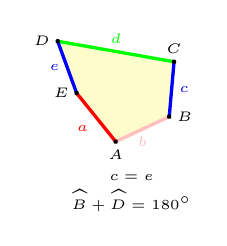
\begin{tikzpicture}[line join=round,line width=1.2pt,scale=.5]
			\begin{tiny}
				\draw (0,0) coordinate (A) node[below] {$A$};
				\draw ($ (A) + (25:15mm) $) coordinate (B) node[right] {$B$};
				\draw ($(B)!14mm!-120:(A)$) coordinate (C) node[above] {$C$};
				\draw ($(C)!30mm!-95:(B)$) coordinate (D) node [left] {$D$};
				\draw ($(D)!14mm!-60:(C)$) coordinate (E) node [left] {$E$};

				\draw[fill=yellow!20,yellow!20] (A) -- (B) -- (C) -- (D) -- (E) -- cycle;


				\draw [pink] (A) -- (B) node[pos=.5,below] {$b$};
				\draw [blue](B) -- (C) node[pos=.5,right] {$c$};
				\draw [green](C) -- (D) node[pos=.5,above] {$d$};
				\draw [blue](D) -- (E) node[pos=.5,left] {$e$};
				\draw[red](E) -- (A) node[pos=.5,below left] {$a$};

				\draw[fill] (A) circle (.6pt);
				\draw[fill] (B) circle (.6pt);
				\draw[fill] (C) circle (.6pt);
				\draw[fill] (D) circle (.6pt);
				\draw[fill] (E) circle (.6pt);


				\draw (.4,-.9) node{$c=e$};
				\draw (.4,-1.5) node{$\widehat{B}+\widehat{D}=180^\circ$};
			\end{tiny}


		\end{tikzpicture}
	};
	\draw (7.5,1.5) node {%
		%%%%%%Pentagon Type 3
		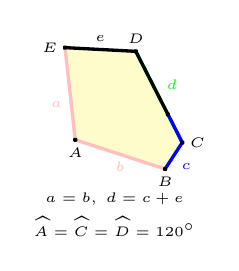
\begin{tikzpicture}[line join=round,line width=1.2pt,scale=.5]
			\begin{tiny}
				\draw (0,0) coordinate (A) node[below] {$A$};
				\draw ($ (A) + (-18:24mm) $) coordinate (B) node[below] {$B$};
				\draw ($(B)!8mm!-105:(A)$) coordinate (C) node[right] {$C$};
				\draw ($(C)!26mm!-120:(B)$) coordinate (D) node [above] {$D$};
				\draw ($(D)!18mm!-120:(C)$) coordinate (E) node [left] {$E$};

				\draw ($(C)!8mm!-120:(B)$) coordinate (BC);



				\draw[fill=yellow!20,yellow!20] (A) -- (B) -- (C) -- (D) -- (E) -- cycle;


				\draw [pink] (A) -- (B) node[pos=.5,below] {$b$};
				\draw [blue](B) -- (C) node[pos=.5,below right] {$c$};
				\draw [green](C) -- (D) node[pos=.5,above right] {$d$};
				\draw (D) -- (E) node[pos=.5,above] {$e$};
				\draw[pink](E) -- (A) node[pos=.5,below left] {$a$};

				\draw[blue] (C) -- (BC);
				\draw (D) -- (BC);

				\draw[fill] (A) circle (.6pt);
				\draw[fill] (B) circle (.6pt);
				\draw[fill] (C) circle (.6pt);
				\draw[fill] (D) circle (.6pt);
				\draw[fill] (E) circle (.6pt);

				\draw[fill] (BC) circle (.6pt);

				\draw (1,-1.5) node{$a=b,\;d=c+e$};
				\draw (1,-2.2) node{$\widehat{A}=\widehat{C}=\widehat{D}=120^\circ$};
			\end{tiny}


		\end{tikzpicture}
	};


	\draw (1.5,4.5) node {%
		%%%%%%Pentagon Type 4
		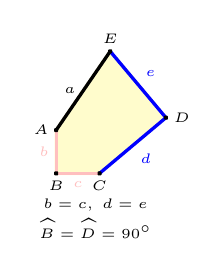
\begin{tikzpicture}[line join=round,line width=1.2pt,scale=.5]
			\begin{tiny}
				\draw (0,0) coordinate (A) node[left] {$A$};
				\draw ($ (A) + (-90:11mm) $) coordinate (B) node[below] {$B$};
				\draw ($(B)!11mm!-90:(A)$) coordinate (C) node[below] {$C$};
				\draw ($(C)!22mm!-140:(B)$) coordinate (D) node [right] {$D$};
				\draw ($(D)!22mm!-90:(C)$) coordinate (E) node [above] {$E$};

				\draw[fill=yellow!20,yellow!20] (A) -- (B) -- (C) -- (D) -- (E) -- cycle;


				\draw [pink] (A) -- (B) node[pos=.5,left] {$b$};
				\draw [pink] (B) -- (C) node[pos=.5,below] {$c$};
				\draw [blue] (C) -- (D) node[pos=.5,below right] {$d$};
				\draw [blue] (D) -- (E) node[pos=.5,above right] {$e$};
				\draw   (E) -- (A) node[pos=.5,left] {$a$};

				\draw[fill] (A) circle (.6pt);
				\draw[fill] (B) circle (.6pt);
				\draw[fill] (C) circle (.6pt);
				\draw[fill] (D) circle (.6pt);
				\draw[fill] (E) circle (.6pt);


				\draw (1,-1.9) node{$b=c,\;d=e$};
				\draw (1,-2.5) node{$\widehat{B}=\widehat{D}=90^\circ$};
			\end{tiny}


		\end{tikzpicture}
	};
	\draw (4.5,4.5) node {%
		%%%%%%Pentagon Type 5
		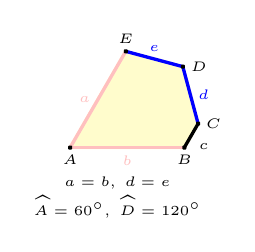
\begin{tikzpicture}[line join=round,line width=1.2pt,scale=.5]
			\begin{tiny}
				\draw (0,0) coordinate (A) node[below] {$A$};
				\draw ($ (A) + (0:29mm) $) coordinate (B) node[below] {$B$};
				\draw ($(B)!7mm!-120:(A)$) coordinate (C) node[right] {$C$};
				\draw ($(C)!15mm!-135:(B)$) coordinate (D) node [right] {$D$};
				\draw ($(D)!15mm!-120:(C)$) coordinate (E) node [above] {$E$};

				\draw[fill=yellow!20,yellow!20] (A) -- (B) -- (C) -- (D) -- (E) -- cycle;


				\draw [pink] (A) -- (B) node[pos=.5,below] {$b$};
				\draw (B) -- (C) node[pos=.5,below right] {$c$};
				\draw [blue](C) -- (D) node[pos=.5,right] {$d$};
				\draw [blue](D) -- (E) node[pos=.5,above] {$e$};
				\draw[pink](E) -- (A) node[pos=.5,left] {$a$};

				\draw[fill] (A) circle (.6pt);
				\draw[fill] (B) circle (.6pt);
				\draw[fill] (C) circle (.6pt);
				\draw[fill] (D) circle (.6pt);
				\draw[fill] (E) circle (.6pt);


				\draw (1.2,-.9) node{$a=b,\;d=e$};
				\draw (1.2,-1.5) node{$\widehat{A}=60^\circ,\;\widehat{D}=120^\circ$};
			\end{tiny}


		\end{tikzpicture}
	};
	\draw (7.5,4.5) node {%
		%%%%%%Pentagon Type 6
		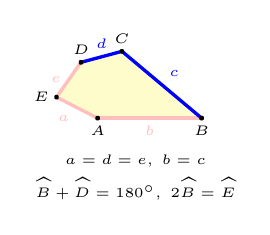
\begin{tikzpicture}[line join=round,line width=1.2pt,scale=.6]
			\begin{tiny}
				\draw (0,0) coordinate (A) node[below] {$A$};
				\draw ($ (A) + (0:22mm) $) coordinate (B) node[below] {$B$};
				\draw ($(B)!22mm!-40:(A)$) coordinate (C) node[above] {$C$};
				\draw ($(C)!9mm!-125:(B)$) coordinate (D) node [above] {$D$};
				\draw ($(D)!9mm!-140:(C)$) coordinate (E) node [left] {$E$};

				\draw[fill=yellow!20,yellow!20] (A) -- (B) -- (C) -- (D) -- (E) -- cycle;


				\draw [pink] (A) -- (B) node[pos=.5,below] {$b$};
				\draw [blue](B) -- (C) node[pos=.5,above right] {$c$};
				\draw [blue](C) -- (D) node[pos=.5,above] {$d$};
				\draw [pink](D) -- (E) node[pos=.5,left] {$e$};
				\draw[pink](E) -- (A) node[pos=.5,below left] {$a$};

				\draw[fill] (A) circle (.6pt);
				\draw[fill] (B) circle (.6pt);
				\draw[fill] (C) circle (.6pt);
				\draw[fill] (D) circle (.6pt);
				\draw[fill] (E) circle (.6pt);


				\draw (.8,-.9) node{$a=d=e,\;b=c$};
				\draw (.8,-1.5) node{$\widehat{B}+\widehat{D}=180^\circ,\;2\widehat{B}=\widehat{E}$};
			\end{tiny}


		\end{tikzpicture}

	};


	\draw (1.5,7.5) node {%
		%%%%%%Pentagon Type 7
		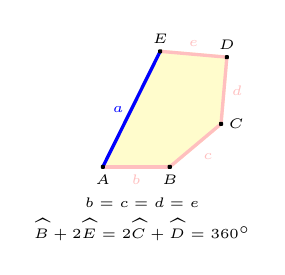
\begin{tikzpicture}[line join=round,line width=1.2pt,scale=.5]
			\begin{tiny}
				\draw (0,0) coordinate (A) node[below] {$A$};
				\draw ($ (A) + (0:17mm) $) coordinate (B) node[below] {$B$};
				\draw ($(B)!17mm!-140:(A)$) coordinate (C) node[right] {$C$};
				\draw ($(C)!17mm!-135:(B)$) coordinate (D) node [above] {$D$};
				\draw ($(D)!17mm!-90:(C)$) coordinate (E) node [above] {$E$};

				\draw[fill=yellow!20,yellow!20] (A) -- (B) -- (C) -- (D) -- (E) -- cycle;


				\draw [pink] (A) -- (B) node[pos=.5,below] {$b$};
				\draw [pink](B) -- (C) node[pos=.5,below right] {$c$};
				\draw [pink](C) -- (D) node[pos=.5,right] {$d$};
				\draw [pink](D) -- (E) node[pos=.5,above] {$e$};
				\draw[blue](E) -- (A) node[pos=.5,left] {$a$};

				\draw[fill] (A) circle (.6pt);
				\draw[fill] (B) circle (.6pt);
				\draw[fill] (C) circle (.6pt);
				\draw[fill] (D) circle (.6pt);
				\draw[fill] (E) circle (.6pt);


				\draw (1,-.9) node{$b=c=d=e$};
				\draw (1,-1.6) node{$\widehat{B}+2\widehat{E}=2\widehat{C}+\widehat{D}=360^\circ$};
			\end{tiny}


		\end{tikzpicture}
	};
	\draw (4.5,7.5) node {%
		%%%%%%Pentagon Type 8
		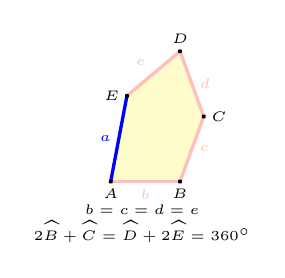
\begin{tikzpicture}[line join=round,line width=1.2pt,scale=.4]
			\begin{tiny}
				\draw (0,0) coordinate (A) node[below] {$A$};
				\draw ($ (A) + (0:22mm) $) coordinate (B) node[below] {$B$};
				\draw ($(B)!22mm!-110:(A)$) coordinate (C) node[right] {$C$};
				\draw ($(C)!22mm!-140:(B)$) coordinate (D) node [above] {$D$};
				\draw ($(D)!22mm!-70:(C)$) coordinate (E) node [left] {$E$};

				\draw[fill=yellow!20,yellow!20] (A) -- (B) -- (C) -- (D) -- (E) -- cycle;


				\draw [pink] (A) -- (B) node[pos=.5,below] {$b$};
				\draw [pink](B) -- (C) node[pos=.5,right] {$c$};
				\draw [pink](C) -- (D) node[pos=.5,right] {$d$};
				\draw [pink](D) -- (E) node[pos=.5,above left] {$e$};
				\draw[blue](E) -- (A) node[pos=.5,left] {$a$};

				\draw[fill] (A) circle (.6pt);
				\draw[fill] (B) circle (.6pt);
				\draw[fill] (C) circle (.6pt);
				\draw[fill] (D) circle (.6pt);
				\draw[fill] (E) circle (.6pt);


				\draw (1,-.9) node{$b=c=d=e$};
				\draw (1,-1.6) node{$2\widehat{B}+\widehat{C}=\widehat{D}+2\widehat{E}=360^\circ$};
			\end{tiny}


		\end{tikzpicture}
	};
	\draw (7.5,7.5) node {%
		%%%%%%Pentagon Type 9
		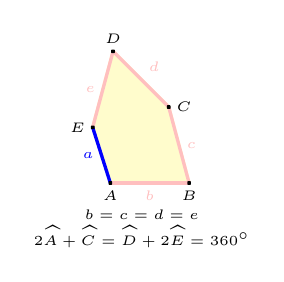
\begin{tikzpicture}[line join=round,line width=1.2pt,scale=.4]
			\begin{tiny}
				\draw (0,0) coordinate (A) node[below] {$A$};
				\draw ($ (A) + (0:25mm) $) coordinate (B) node[below] {$B$};
				\draw ($(B)!25mm!-75:(A)$) coordinate (C) node[right] {$C$};
				\draw ($(C)!25mm!-150:(B)$) coordinate (D) node [above] {$D$};
				\draw ($(D)!25mm!-60:(C)$) coordinate (E) node [left] {$E$};

				\draw[fill=yellow!20,yellow!20] (A) -- (B) -- (C) -- (D) -- (E) -- cycle;


				\draw [pink] (A) -- (B) node[pos=.5,below] {$b$};
				\draw [pink](B) -- (C) node[pos=.5,right] {$c$};
				\draw [pink](C) -- (D) node[pos=.5,above right] {$d$};
				\draw [pink](D) -- (E) node[pos=.5,left] {$e$};
				\draw[blue](E) -- (A) node[pos=.5,left] {$a$};

				\draw[fill] (A) circle (.6pt);
				\draw[fill] (B) circle (.6pt);
				\draw[fill] (C) circle (.6pt);
				\draw[fill] (D) circle (.6pt);
				\draw[fill] (E) circle (.6pt);


				\draw (1,-1) node{$b=c=d=e$};
				\draw (1,-1.7) node{$2\widehat{A}+\widehat{C}=\widehat{D}+2\widehat{E}=360^\circ$};
			\end{tiny}


		\end{tikzpicture}
	};


	\draw (1.5,10.5) node {%
		%%%%%%Pentagon Type 10
		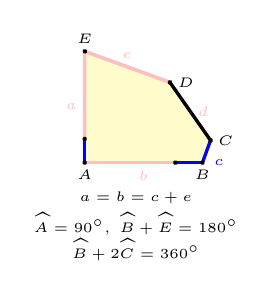
\begin{tikzpicture}[line join=round,line width=1.2pt,scale=.5]
			\begin{tiny}
				\draw (0,0) coordinate (A) node[below] {$A$};
				\draw ($ (A) + (0:29.9mm) $) coordinate (B) node[below] {$B$};
				\draw ($(B)!6mm!-110:(A)$) coordinate (C) node[right] {$C$};
				\draw ($(C)!18mm!-125:(B)$) coordinate (D) node [right] {$D$};
				\draw ($(D)!23mm!-145:(C)$) coordinate (E) node [above] {$E$};

				\draw ($ (A) + (0:23mm) $) coordinate (AA);
				\draw ($(A) + (90:6mm)$) coordinate (EE);

				\draw[fill=yellow!20,yellow!20] (A) -- (B) -- (C) -- (D) -- (E) -- cycle;


				\draw [pink] (A) -- (B) node[pos=.5,below] {$b$};
				\draw [blue](B) -- (C) node[pos=.5,below right] {$c$};
				\draw [pink](C) -- (D) node[pos=.5,right] {$d$};
				\draw [pink](D) -- (E) node[pos=.5,above] {$e$};
				\draw[white](E) -- (A) node[pos=.5,left] {\color{pink} $a$};


				\draw[pink] (A) -- (AA);
				\draw[blue] (B) -- (AA);
				\draw (C) -- (D);
				\draw[pink] (D) -- (E);
				\draw[pink] (E) -- (EE);
				\draw[blue] (A) -- (EE);

				\draw[fill] (A) circle (.6pt);
				\draw[fill] (B) circle (.6pt);
				\draw[fill] (C) circle (.6pt);
				\draw[fill] (D) circle (.6pt);
				\draw[fill] (E) circle (.6pt);

				\draw[fill] (AA) circle (.6pt);
				\draw[fill] (EE) circle (.6pt);

				\draw (1.3,-.9) node{$a=b=c+e$};
				\draw (1.3,-1.55) node{$\widehat{A}=90^\circ,\;\widehat{B}+\widehat{E}=180^\circ$};
				\draw (1.3,-2.2) node{
					$\widehat{B}+2\widehat{C}=360^\circ$};
			\end{tiny}


		\end{tikzpicture}

	};
	\draw (4.5,10.5) node {%
		%%%%%%Pentagon Type 11
		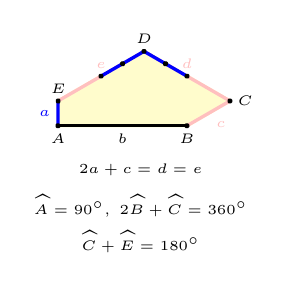
\begin{tikzpicture}[line join=round,line width=1.2pt,scale=.7]
			\begin{tiny}
				\draw (0,0) coordinate (A) node[below] {$A$};
				\draw ($ (A) + (0:23.4mm) $) coordinate (B) node[below] {$B$};
				\draw ($(B)!9mm!-150:(A)$) coordinate (C) node[right] {$C$};
				\draw ($(C)!18mm!-60:(B)$) coordinate (D) node [above] {$D$};
				\draw ($(D)!18mm!-120:(C)$) coordinate (E) node [above] {$E$};


				\draw ($(C)!9mm!-60:(B)$) coordinate (CC);
				\draw ($(CC)!4.5mm!0:(D)$ ) coordinate (CCC);
				\draw ($(D)!4.5mm!0:(E)$) coordinate (DD);
				\draw ($(DD)!4.5mm!0:(E)$) coordinate (DDD);



				\draw[fill=yellow!20,yellow!20] (A) -- (B) -- (C) -- (D) -- (E) -- cycle;


				\draw (A) -- (B) node[pos=.5,below] {$b$};
				\draw [pink](B) -- (C) node[pos=.5,below right] {$c$};
				\draw [pink](C) -- (D) node[pos=.5,above] {$d$};
				\draw [pink](D) -- (E) node[pos=.5,above] {$e$};
				\draw[blue](E) -- (A) node[pos=.5,left] {$a$};


				\draw[blue] (D) -- (DD);
				\draw[blue] (DDD) -- (DD);
				\draw[blue] (CC) -- (CCC);
				\draw[blue] (CCC) -- (D);


				\draw[fill] (A) circle (.6pt);
				\draw[fill] (B) circle (.6pt);
				\draw[fill] (C) circle (.6pt);
				\draw[fill] (D) circle (.6pt);
				\draw[fill] (E) circle (.6pt);






				\draw[fill] (CC) circle (.6pt);
				\draw[fill] (CCC) circle (.6pt);
				\draw[fill] (DD) circle (.6pt);
				\draw[fill] (DDD) circle (.6pt);



				\draw (1.5,-.8) node {$2a+c=d=e$ };
				\draw (1.5,-1.45) node {$\widehat{A}=90^\circ,\;2\widehat{B}+\widehat{C}=360^\circ$};
				\draw (1.5,-2.1) node {$\widehat{C}+\widehat{E}=180^\circ$};
			\end{tiny}


		\end{tikzpicture}
	};
	\draw (7.5,10.5) node {%
		%%%%%%Pentagon Type 12
		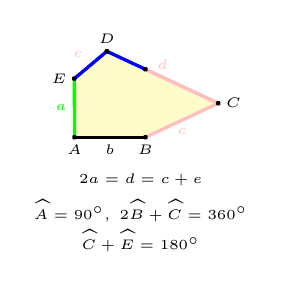
\begin{tikzpicture}[line join=round,line width=1.2pt,scale=.6]
			\begin{tiny}
				\draw (0,0) coordinate (A) node[below] {$A$};
				\draw ($ (A) + (0:15mm) $) coordinate (B) node[below] {$B$};
				\draw ($(B)!17mm!-155:(A)$) coordinate (C) node[right] {$C$};
				\draw ($(C)!26mm!-50:(B)$) coordinate (D) node [above] {$D$};
				\draw ($(D)!9mm!-115:(C)$) coordinate (E) node [left] {$E$};

				\draw ($(C)!17mm! 0:(D)$) coordinate (CC);


				\draw[fill=yellow!20,yellow!20] (A) -- (B) -- (C) -- (D) -- (E) -- cycle;


				\draw  (A) -- (B) node[pos=.5,below] {$b$};
				\draw [pink](B) -- (C) node[pos=.5,below] {$c$};
				\draw [pink](C) -- (D) node[pos=.5,above] {$d$};
				\draw [pink](D) -- (E) node[pos=.5,above left] {$e$};
				\draw[green](E) -- (A) node[pos=.5,left] {$a$};

				\draw[pink] (C) -- (CC);
				\draw[blue] (CC) -- (D);
				\draw[blue] (D) -- (E);


				\draw[fill] (A) circle (.6pt);
				\draw[fill] (B) circle (.6pt);
				\draw[fill] (C) circle (.6pt);
				\draw[fill] (D) circle (.6pt);
				\draw[fill] (E) circle (.6pt);

				\draw[fill] (CC) circle (.6pt);

				\draw (1.4,-.9) node{$2a=d=c+e$};
				\draw (1.4,-1.55) node{$\widehat{A}=90^\circ,\;2\widehat{B}+\widehat{C}=360^\circ$};
				\draw (1.4,-2.2) node{$\widehat{C}+\widehat{E}=180^\circ$};
			\end{tiny}


		\end{tikzpicture}
	};


	\draw (1.5,13.5) node {%
		%%%%%%Pentagon Type 13
		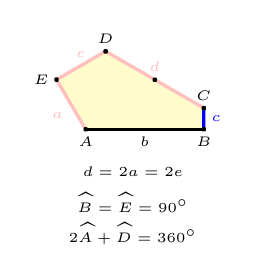
\begin{tikzpicture}[line join=round,line width=1.2pt,scale=.6]
			\begin{tiny}
				\draw (0,0) coordinate (A) node[below] {$A$};
				\draw ($ (A) + (0:25mm) $) coordinate (B) node[below] {$B$};
				\draw ($(B)!4.5mm!-90:(A)$) coordinate (C) node[above] {$C$};
				\draw ($(C)!24mm!-120:(B)$) coordinate (D) node [above] {$D$};
				\draw ($(D)!12mm!-120:(C)$) coordinate (E) node [left] {$E$};

				\draw ($(C)!12mm!0:(D)$) coordinate (CC);

				\draw[fill=yellow!20,yellow!20] (A) -- (B) -- (C) -- (D) -- (E) -- cycle;


				\draw  (A) -- (B) node[pos=.5,below] {$b$};
				\draw [blue](B) -- (C) node[pos=.5,right] {$c$};
				\draw [pink](C) -- (D) node[pos=.5,above] {$d$};
				\draw [pink](D) -- (E) node[pos=.5,above] {$e$};
				\draw[pink](E) -- (A) node[pos=.5,below left] {$a$};

				\draw[fill] (A) circle (.6pt);
				\draw[fill] (B) circle (.6pt);
				\draw[fill] (C) circle (.6pt);
				\draw[fill] (D) circle (.6pt);
				\draw[fill] (E) circle (.6pt);

				\draw[fill] (CC) circle (.6pt);

				\draw (1,-.9) node{$d=2a=2e$};
				\draw (1,-1.55) node{$\widehat{B}=\widehat{E}=90^\circ$};
				\draw (1,-2.2) node{$2\widehat{A}+\widehat{D}=360^\circ$};
			\end{tiny}


		\end{tikzpicture}
	};
	\draw (4.5,13.5) node {%
		%%%%%%Pentagon Type 14
		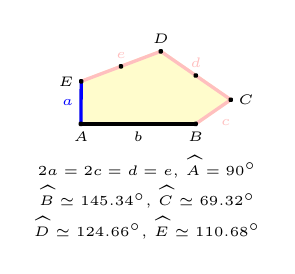
\begin{tikzpicture}[line join=round,line width=1.2pt,scale=.6]
			\begin{tiny}
				\draw (0,0) coordinate (A) node[below] {$A$};
				\draw ($ (A) + (0:24.3mm) $) coordinate (B) node[below] {$B$};
				\draw ($(B)!9mm!-145.34:(A)$) coordinate (C) node[right] {$C$};
				\draw ($(C)!18mm!-69.32:(B)$) coordinate (D) node [above] {$D$};
				\draw ($(D)!18mm!-124.66:(C)$) coordinate (E) node [left] {$E$};

				\draw[fill=yellow!20,yellow!20] (A) -- (B) -- (C) -- (D) -- (E) -- cycle;

				\draw ($(E)!9mm!0:(D)$) coordinate (EE);
				\draw ($(D)!9mm!0:(C)$) coordinate (DD);

				\draw (A) -- (B) node[pos=.5,below] {$b$};
				\draw [pink](B) -- (C) node[pos=.5,below right] {$c$};
				\draw [pink](C) -- (D) node[pos=.5,above] {$d$};
				\draw [pink](D) -- (E) node[pos=.5,above] {$e$};
				\draw[blue](E) -- (A) node[pos=.5,left] {$a$};

				\draw[fill] (A) circle (.6pt);
				\draw[fill] (B) circle (.6pt);
				\draw[fill] (C) circle (.6pt);
				\draw[fill] (D) circle (.6pt);
				\draw[fill] (E) circle (.6pt);

				\draw[fill] (EE) circle (.6pt);
				\draw[fill] (DD) circle (.6pt);


				\draw (1.4,-.9) node{$2a=2c=d=e,\,\widehat{A}=90^\circ$};
				\draw (1.4,-1.55) node{$\widehat{B}\simeq 145.34^\circ,\,
						\widehat{C}\simeq 69.32^\circ$};
				\draw (1.4,-2.2) node{$
						\widehat{D}\simeq 124.66^\circ,\,
						\widehat{E}\simeq 110.68^\circ$
					%%(2\widehat{B}+\widehat{C}=360^\circ,\; \widehat{C}+\widehat{E}=180^\circ)
				};
			\end{tiny}


		\end{tikzpicture}
	};
	\draw (7.5,13.5) node {%
		%%%%%%Pentagon Type 15
		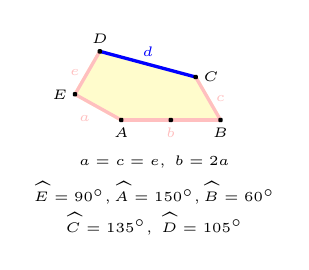
\begin{tikzpicture}[line join=round,line width=1.2pt,scale=.6]
			\begin{tiny}
				\draw (0,0) coordinate (A) node[below] {$A$};
				\draw ($ (A) + (0:21mm) $) coordinate (B) node[below] {$B$};
				\draw ($(B)!10.5mm!-60:(A)$) coordinate (C) node[right] {$C$};
				\draw ($(C)!21mm!-135:(B)$) coordinate (D) node [above] {$D$};
				\draw ($(D)!10.5mm!-105:(C)$) coordinate (E) node [left] {$E$};

				\draw ($(A)!10.5mm!0:(B)$) coordinate (AA);


				\draw[fill=yellow!20,yellow!20] (A) -- (B) -- (C) -- (D) -- (E) -- cycle;


				\draw [pink] (A) -- (B) node[pos=.5,below] {$b$};
				\draw [pink](B) -- (C) node[pos=.5,right] {$c$};
				\draw [blue](C) -- (D) node[pos=.5,above] {$d$};
				\draw [pink](D) -- (E) node[pos=.5,left] {$e$};
				\draw[pink](E) -- (A) node[pos=.5,below left] {$a$};

				\draw[fill] (A) circle (.6pt);
				\draw[fill] (B) circle (.6pt);
				\draw[fill] (C) circle (.6pt);
				\draw[fill] (D) circle (.6pt);
				\draw[fill] (E) circle (.6pt);

				\draw[fill] (AA) circle (.6pt);

				\draw (.7,-.9) node{$a=c=e,\;b=2a$};
				\draw (.7,-1.55) node{$
						\widehat{E}=90^\circ,
						\widehat{A}=150^\circ,
						\widehat{B}=60^\circ$};
				\draw (.7,-2.2) node{$
						\widehat{C}=135^\circ,\;\widehat{D}=105^\circ$};
			\end{tiny}
		\end{tikzpicture}
	};
\end{tikzpicture}

\end{document}
